%======================================================================
\chapter{Software Implementation (MOUSE)}
%======================================================================

The Modular autOmated Up-Scaling softwarE (MOUSE) for DEM simulations was created and written in Python\textsuperscript{TM} to provide an implementation of the up-scaling framework presented in the previous chapter using third-party software. The software itself aims to provide a platform through which the four software elements of the up-scaling framework (DEM, homogenization, parameter estimation, and macroscale model) can communicate with each other. The communication is facilitated by MOUSE through modules which wrap the third party software in such a way that the inputs and outputs to and from the modules are in a consistent structure regardless of the third party software being used. 

This chapter of the thesis aims to provide a very high level overview of the key aspects of the MOUSE software implementation without getting into any of the fine details. The programatic structure of some of the important software components is presented to illustrate the software design, but a complete discussion on the construction of all the specific wrappers gets unweildly.

The general idea with the up-scaling framework developed in this thesis is that it is model independant. Because of this, it is important that MOUSE was written in such a way that allowed for different models (both DEM and macroscale) to be implemented without rewriting the up-scaling algorithms. As such, a modular approach was taken such that each module is isolated from the others and only communicates data through strict protocols set out by MOUSE.

There exists four base classes that are used as parents to the third-party software module classes. Because each software compent has distinct I/O protocols, the base classes serve as a collection of usefull methods which the software module can inherit to ensure compatibility with MOUSE. Each of these four component base classes inherit from a base module class. Figure \ref{fig:moduleClass} indicates this class heirarchy as well as where each method and attribute definition falls in the heirarchy.

\begin{figure}[!htb]
\begin{center}
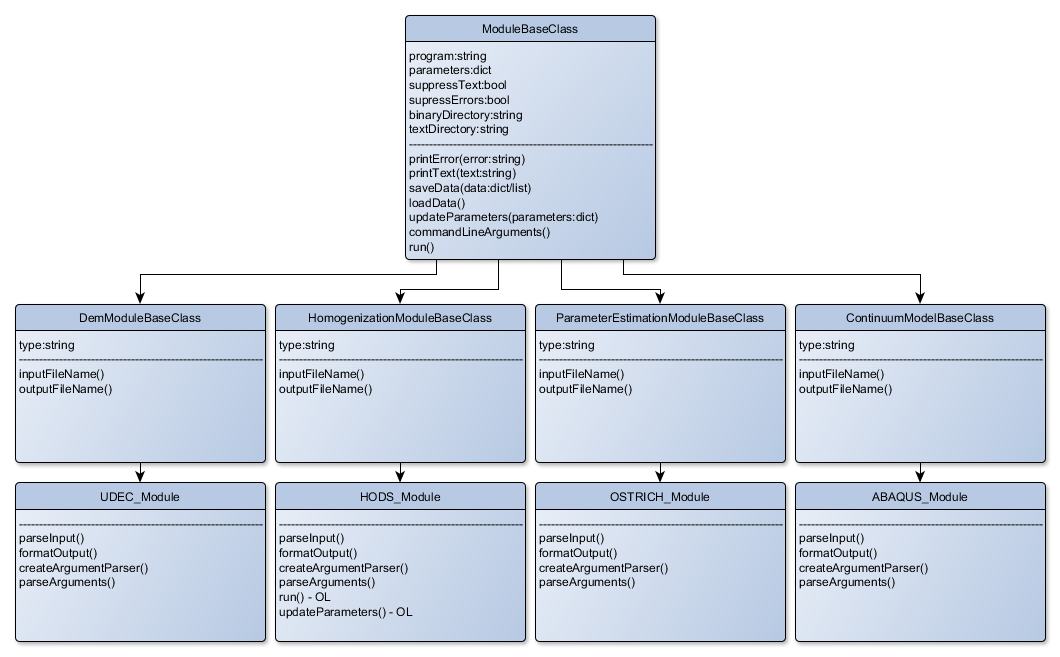
\includegraphics[width=\textwidth]{figures/Chapter4/ModuleClassUML}
\caption{{\label{fig:moduleClass} Module class inheritence structure.%
}}
\end{center}
\end{figure}

%----------------------------------------------------------------------
\section{Base Module Class}
%----------------------------------------------------------------------

A base module class, \textbf{BaseModuleClass}, is implemented to provide a framework containing required methods and attributes for the MOUSE modules to inherit. The module class contains methods pertaining to I/O routines associated with the module so that each module that is written behaves in a consistent manner and to avoid reimplementation of certain methods. 

\subsection{Attributes}

Attributes are assigned to \textbf{BaseModuleClass} through the constructor method (\textbf{\_\_init\_\_}) when the class is initialized. The following attributes are passed as arguments through instantiation of the class children. 

The \textbf{program} attribute is a string that contains the name of the software excecutable associated with the given module. This parmeter allows the module the capacity to run the program through a command line interface (CLI) As such, the program must be able to accept command line arguments.

\begin{lstlisting}[frame=single]  
#String containing name of module software executable file. 
self.program = program
\end{lstlisting}

The \textbf{parameters} attribute is a dictionary that contains all the command line parameters and corresponding arguments. Here, the parameters are the dictionary keys and the arguments are the dictionary values. If no arguments are required, then an empty dictionary is acceptable aswell. 

\begin{lstlisting}[frame=single]   
#Dictionary of command line parameters and corresponding arguments
self.parameters = parameters
\end{lstlisting}

The \textbf{supressText} and \textbf{supressErrors} attributes are Boolean parameters that, when true, allow for the suppression of command line output of text and errors, respectively.

\begin{lstlisting}[frame=single]   
#Boolean parameter that allows text output to CMD to be supressed
self.suppressText = suppressText

#Boolean parameter that allows errors to be supressed
self.suppressErrors = suppressErrors
\end{lstlisting}

The \textbf{binaryDirectory} and \textbf{textDirectory} attributes are strings that refer to file folders in which the binary and text data are to be saved, respectively. these values are determined through relative directory parsing, rather than as an initialization argument. \\\\

\begin{lstlisting}[frame=single]   	
#String that indicates where to store the binary data
self.binaryDirectory = os.path.join(dataDirectory, 'Binary')

#String that indicates where to store the text data
self.textDirectory = os.path.join(dataDirectory, 'Text')
\end{lstlisting}


\subsection{Defined Methods}
Methods in \textbf{BaseModuleClass} are divided into two types: defined and undefined. Defined methods are methods that are common to all the module classes and are thus able to be defined at the parent level. The undefined methods are methods that require overloading, so they are defined at the child level. 

The \textbf{\_\_init\_\_} method is a built-in contructor method that is automatically called when the class is initialized. The only required argument for this method is \textbf{parameter}, with the other three being optional arguments. 

\begin{lstlisting}[frame=single]
#Contructor method that is called when the class is initialized
def __init__(self, program, parameters={}, suppressText=False, suppressErrors=True):
	"""
	program:	string of program name
	parameters:	dictionary of parameter-argument pairs
	suppressText:	boolean
	suppressErrors:	boolean"""
	
\end{lstlisting}

A series of printing methods are included in \textbf{BaseModuleClass} to allow each module to route command line output through the parent module for consistent output formatting. The \textbf{printText}, \textbf{printTitle}, \textbf{printSection}, \textbf{printStatus}, \textbf{printDone}, and \textbf{printErrors} methods are implemented to give a large degree of flexibility in the displayed output.

\begin{lstlisting}[frame=single]
#Method to print text to command line if text supression is off
def printText(self, text):
	"""
	text:		string of text to print """
	
#Method to format primary title in command line output 
def printTitle(self, title):
	"""
	title:		string of primary title to print"""
	
#Method to format section title in command line output 
def printSection(self, section):
	"""
	section:	string of section title to print"""
	
#Method to format status update in command line output 
def printStatus(self, status):
	"""
	status:		string of status to print"""
	
#Method to print 'Done' when section is finished 
def printDone(self):
	"""	
	"""
	
#Method to control and print errors if error supression is off
def printErrors(self, error):
	"""
	error:		error to print"""
\end{lstlisting}

The \textbf{saveData} and \textbf{loadData} methods use binary serialization methods to write and load specified data structures to and from file. Saving and loading serialized binary data is much faster and more compact than unicode.

\begin{lstlisting}[frame=single]        
#Method to save serialized data structures as output
def saveData(self, data):
	"""
	data:		Data format specified by module type"""
	
#Method to load serialized data structures as input
def loadData(self):
	"""
	"""
\end{lstlisting}

The \textbf{updateParameters} method allows for the dynamic updating of module input parameters. This allows for the module to run the program multiple times without being reinstantiated.

\begin{lstlisting}[frame=single]    
#Method that allows dynamic updating of parameters.
def updateParameters(self, parameters):
	"""
	parameters:	dictionary of parameter-argument pairs	"""
\end{lstlisting}

The \textbf{commandLineArguments} method takes the \textbf{parameters} dictionary attribute and converts it to a string which can be passed to the command line when running the specified program.

\begin{lstlisting}[frame=single]
#Method to create a string of command line arguments from parameters
def commandLineArguments(self):
	"""
	"""
\end{lstlisting}

The \textbf{run} method simply runs the specified program with the specified parameters. 

\begin{lstlisting}[frame=single]    
#Method to run the program with the specified parameters
def run(self):
	"""
	"""
\end{lstlisting}

\subsection{Undefined Methods}

The undefined methods listed here are required to be defined in the child classes. These methods are different for each type of module or even each module implementation, which does not allow them to be written in \textbf{baseModuleClass}. 

The \textbf{createArgumentParser} method creates an argument parser that allows the module to parse any command line arguments passed to it if the module is run in an isolated environment, While the \textbf{parseArguments} method parses the command line arguments derived from \textbf{createArgumentParser}.

\begin{lstlisting}[frame=single]    
def createArgumentParser(self):
    
def parseArguments(self):
\end{lstlisting}

The \textbf{inputFileName} and \textbf{outputFileName} methods provide the formatting for the fileNames in a means that is consistent amongst modules.

\begin{lstlisting}[frame=single]
def inputFileName(self):
        
def outputFileName(self):
\end{lstlisting}

%----------------------------------------------------------------------
\section{Data Architechture}
%----------------------------------------------------------------------

This section aims to explain the data structures used to store and transfer data between the modules in the up-scaling framework presented in this thesis.  Three fundamental data structures are used for the storage of data in conjunction with each other: hash tables, lists, and arrays. Using these three structures, three distinct types of data in the up-scaling framework are used to transfer between the modules in a consistent manner: constitutive parameters, DEM data, and continuum data.

\subsubsection*{Python Lists}

The list in Python\textsuperscript{TM} is one of the most versatile data structures. The list treats the data as a sequence such that each element in the list is assigned a number referring to its position or index.  The implementation of the list structure in python contains a number of unique features. The main feature of python lists is that the elements within the lists are not required to be of the same data type. Additionally, these lists are mutable, allowing for more advanced manipulation of the data structure. Because of this flexibility, the list structure is slow and unsuitable for large data sets. 

\subsubsection*{Numpy Arrays}

Numpy arrays are a specific implementation of a python list which are optimized for numerical operations on large datasets. Here the numpy arrays are much more compact by using a sequence of uniform values, rather than a sequence of pointers as is the case for the list structure.

\subsubsection*{Python Dictionaries (Hash Tables)}

In general, a hash table is a data structure that maps keys to values. The implementation of hash tables in Python\textsuperscript{TM}, are referred to as dictionaries. Similar to a python list, a python dictionary is a mutable structure that does not require the elements to be of the same type. However, instead of accessing the element value through an index argument, the data is accessed through a key argument. This unordered structure is usefull for storing non-sequential data.

\subsection{Data Storage Structures}

Three distinct types of data are used in the information tranfer protocols between modules: constitutive parameter data, DEM data, and continuum data. these different types fo data require different data structure which are explained in more detail below. The constitutive parameter data is stored in a hash table, the DEM data is stored in a three level nested hash table, and the continuum data is stored in a list of arrays.

\subsubsection*{Hash Tables for Constitutive Parameters}

Constitutive parameters are required as an input to the DEM and macroscale modules as well as an output from the parameter estimation module. Here, the constutive parameters are always stored in a Python\textsuperscript{TM} dictionary with the constitutive parameter name as the key. To access the value of a specific constitutive parameter in a dictionary named 'constitutiveParameters', the string corresponding to the 

\begin{lstlisting}[frame=single]
parameterValue = constitutiveParameters[parameterName]
\end{lstlisting}

For example, accessing the value of the elastic modulus from a hash table named 'contitutiveParameters' is performed as follows:

\begin{lstlisting}[frame=single]
elasticModulus = constitutiveParameters['elasticModulus']
\end{lstlisting}

\subsubsection*{Nested Hash Tables for DEM Data}
The raw DEM Data is considered to be comprised of six distinct types: block data, contact data, corner data, domain data, grid point data, and zone data. Here, each block, contact, corner, domain, grid point, and zone is assigned a unique 7 digit numeric identifier (assuming here that the number of components in the system does not exceed 10 million) by which the associated data can be accessed. The same identifier may be repeated for different data types.

To allow for convenient access to the data, the DEM data is stored in six distinct nested hash tables corresponding to each of the DEM data types.  Each DEM data hash table has three levels of nesting. The first level keys are the simulation times, which returns the second level of hash tables. The second level keys are the component identifiers, which returns a third level hash table. In this third level, the component attirbutes can be accessed using the attirbute name as the key. In general, accessing an attribute of a specific component with a given ID at a specific time from a hash table called demDataHash is done as follows:


\begin{lstlisting}[frame=single]
componentAttributeValue = demDataHash[time][ID][attribute]
\end{lstlisting}

For example, accessing the list of grid points associatied with block ID 2543465 at a simulation time of 1 is performed as follows:

\begin{lstlisting}[frame=single]
gridPoints = blockData[1.0][2543465]['gridPoints']
\end{lstlisting}

The keys of each of the third level dictionaries for each comonent are presented in Table \ref{tab:keys1}, Table \ref{tab:keys2}, Table \ref{tab:keys3}, Table \ref{tab:keys4}, Table \ref{tab:keys5}, and Table \ref{tab:keys6} for the block data, contact data, corner data, domain data, gridpoint data, and zone data, respectively.

\begin{table}[!htb]
\centering
\caption{{Block data attributes in third level hash}}
\label{tab:keys1}
\begin{tabularx}{\textwidth}{@{}Yp{0.75\textwidth}@{}}
\toprule
\textbf{Parameter} & \textbf{Description (Data Type)}                            \\ \midrule
x                  & X coordinate of block centroid (float)                      \\
y                  & Y coordinate of block centroid (float)                      \\
xForce             & Resultant forces at block centroid (float)                  \\
yForce             & Resultant forces at block centroid (float)                  \\
corners            & Corners associated with this block (list of corner IDs)     \\
zones              & Zones associated with this block (list of zone IDs)         \\
gridPoints         & Grid points associated with this block (list of corner IDs) \\ \bottomrule
\end{tabularx}
\end{table}

\begin{table}[!htb]
\centering
\caption{{Contact data attributes in third level hash}}
\label{tab:keys2}
\begin{tabularx}{\textwidth}{@{}Yp{0.75\textwidth}@{}}
\toprule
\textbf{Parameter} & \textbf{Description (Data Type)}                          \\ \midrule
x                  & X coordinate of contact point (float)                     \\
y                  & Y coordinate of contact point (float)                     \\
length             & Length associated with contact point (float)              \\
flowRate           & Fluid flow rate through contact (float)                   \\
nForce             & Resultant normal force on contact (float)                 \\
sForce             & Resultant shear force on contact (float)                  \\
xCosine            & X component of contact normal cosine (float)              \\
yCosine            & Y component of contact normal cosine (float)              \\
blocks             & Blocks associated with this contact (list of block IDs)   \\
domains            & Domains associated with this contact (list of domain IDs) \\
corners            & Corners associated with this contact (list of corner IDs) \\ \bottomrule
\end{tabularx}
\end{table}

\begin{table}[!htb]
\centering
\caption{Corner data attributes in third level hash}
\label{tab:keys3}
\begin{tabularx}{\textwidth}{@{}Yp{0.75\textwidth}@{}}
\toprule
\textbf{Parameter} & \textbf{Description (Data Type)}                                 \\ \midrule
gridPoint          & Grid points associated with this corner (list of grid point IDs) \\ \bottomrule
\end{tabularx}
\end{table}

\begin{table}[!htb]
\centering
\caption{Domain data attributes in third level hash}
\label{tab:keys4}
\begin{tabularx}{\textwidth}{@{}Yp{0.75\textwidth}@{}}
\toprule
\textbf{Parameter} & \textbf{Description (Data Type)}            \\ \midrule
x       & X coordinate of domain centroid (float)     \\
y       & Y coordinate of domain centroid (float)     \\
area               & Area of domain (float)                      \\
porePressure      & Average pore pressure in the domain (float)\\ \bottomrule
\end{tabularx}
\end{table}

\begin{table}[!htb]
\centering
\caption{Gridpoint data attributes in third level hash}
\label{tab:keys5}
\begin{tabularx}{\textwidth}{@{}Yp{0.75\textwidth}@{}}
\toprule
\textbf{Parameter} & \textbf{Description (Data Type)}                             \\ \midrule
x       & X coordinate of grid point (float)                           \\
y       & Y coordinate of grid point (float)                           \\
xDisp     & X displacement of grid point (float)                         \\
yDisp     & Y displacement of grid point (float)                         \\
xForce            & Resultant X force on grid point (float)                      \\
yForce            & Resultant Y force on grid point (float)                      \\
xVel         & X velocity of grid point (float)                             \\
yVel         & Y velocity of grid point (float)                             \\
block              & Block associated with this grid point (block ID)   \\
corner             & Corner associated with this grid point (corner ID)\\ \bottomrule
\end{tabularx}
\end{table}

\begin{table}[!htb]
\centering
\caption{Zone data attributes in third level hash}
\label{tab:keys6}
\begin{tabularx}{\textwidth}{@{}Yp{0.75\textwidth}@{}}
\toprule
\textbf{Parameter} & \textbf{Description (Data Type)}                                \\ \midrule
S11                & X component of stress in the zone (float)                       \\
S22                & Y component of stress in the zone (float)                       \\
S12                & Corresponding shear stress in the zone (float)                  \\
block              & Block associated with this zone (block ID)                      \\
gridPoints         & Grid points associated with this grid point (list of block IDs)\\ \bottomrule
\end{tabularx}
\end{table}

\subsubsection*{Nested List of Arrays for Continuum Data}

The continuum data is stored in three lists: a normal list and two nested lists of arrays. The three lists contain the time data, stress data, and strain data. The time data is in the normal list, with each element representing a different time step. The other two lists contain two-dimensional nested arrays representing the stress and strain tensors respectively. Each array element within within these lists represents the stress or strain tensors for the corresponding timestep.

\subsection{Binary Serialization}

These data structures mentioned above are great for efficiently accessing the desired data, but cannot easily be saved to file in standard unicode. In the event that this is possible, formatting and parsing large data sets from file becomes slow and increases the possibility of data corruption. To speed up the data access and increase the integrity of the data, binary serialization is employed. 

Binary serialization stores the state of any given object by converting the public and private fields of the class to a stream of bytes, which is then written to the data stream. This data stream can easily be written to a binary file and subsequently read at any later date. The deserialization of this data stream takes the stream of bytes and reconstructs an exact clone of the original object whenever it is required. This method is usefull when attemping to store large non-linear data structures to file.


%----------------------------------------------------------------------
% \section{Specific Module Implementation}
%----------------------------------------------------------------------
% ***
% \subsection{UDEC Module}
% ***
% \subsection{HODS Module}
% ***
% \subsection{OSTRICH Module}
% ***
% \subsection{ABAQUS Module}
% ***


%----------------------------------------------------------------------
\section{HODS Homogenization}
%----------------------------------------------------------------------

HODS homogeniziation module....
\subsection{Class Attributes}


\begin{lstlisting}[frame=single] 
self.fileName = fileName
\end{lstlisting}


\begin{lstlisting}[frame=single] 
self.centre = centre
self.radius = radius
\end{lstlisting}


\begin{lstlisting}[frame=single] 
self.blockData = self.parseDataFile(blockFileName)
self.contactData = self.parseDataFile(contactFileName)
self.cornerData = self.parseDataFile(cornerFileName)
self.zoneData = self.parseDataFile(zoneFileName)
self.gridPointData = self.parseDataFile(gridPointFileName)
self.domainData = self.parseDataFile(domainFileName)
\end{lstlisting}


\begin{lstlisting}[frame=single] 
self.boundaryBlocks = self.blocksOnBoundary()
self.insideBlocks = self.blocksInsideBoundary()
self.outsideBlocks = self.blocksOutsideBoundary()
self.insideBoundaryBlocks = self.boundaryBlocks + self.insideBlocks
self.boundaryContacts = self.contactsBetweenBlocks(self.outsideBlocks, self.boundaryBlocks)
self.boundaryContactCorners = self.cornersOnContacts(self.boundaryContacts)
self.boundaryContactBlocks = self.blocksWithContacts(self.boundaryBlocks, self.boundaryContacts)
self.outsideCorners = self.cornersOutsideBoundary()
self.outsideContacts = self.contactsOutsideBoundary()
self.boundaryBlockCorners = self.cornersOnBlocks(self.boundaryContactBlocks)
self.boundaryCorners = common.listIntersection(self.boundaryContactCorners, self.boundaryBlockCorners)
self.allBoundaryCorners = self.boundaryCorners
self.boundaryBlocksOrdered = self.orderBlocks(self.boundaryContactBlocks, self.outsideContacts)
self.boundaryCornersOrdered = self.orderCorners(self.boundaryBlocksOrdered, self.allBoundaryCorners)
\end{lstlisting}

\subsection{Class Data Methods}

\begin{lstlisting}[frame=single] 
def parseDataFile(self, fileName):
	"""
	fileName:	Name of file that contains DEM data
	"""
	return data
\end{lstlisting}

\begin{lstlisting}[frame=single] 
def cornersOnContacts(self, contacts):
	"""
	contacts:	list of contact IDs
	"""
	return corners

def zonesInBlocks(self, blocks):
	"""
	blocks:		list of block IDs
	"""
	return zones

def cornersOnBlocks(self, blocks):
	"""
	blocks:		list of block IDs
	"""
	return corners

def contactsOnBlocks(self, blocks):
	"""
	blocks:		list of block IDs
	"""
	return contacts
\end{lstlisting}

\begin{lstlisting}[frame=single] 
def contactsBetweenBlocks(self, blocks1, blocks2):
	"""
	blocks1:	list of block IDs
	blocks2: 	list of block IDs
	"""
	return contacts

def blocksWithContacts(self, blocks, contacts):
	"""
	blocks:		list of block IDs
	contacts:	list of contact IDs
	"""
	return newBlocks

def blocksWithCorners(self, blocks, corners):
	"""
	blocks:		list of block IDs
	corners:	list of corner IDs
	"""
	return newBlocks
	
def orderBlocks(self, blocks, relaventContacts):
	"""
	blocks:		list of block IDs
	relContacts:	list of contact IDs
	"""
	return orderedBlocks
	
def orderCorners(self, orderedBlocks, corners):
	"""
	orderedBlocks:	list of block IDs
	corners:	list of corner IDs
	"""
	return orderedCorners
\end{lstlisting}
	
\subsection{Class Boundary Methods}

\begin{lstlisting}[frame=single] 
def blocksOnBoundary(self):
	"""
	"""
	return blocks

def blocksOutsideBoundary(self):
	"""
	"""
	return blocks
        
def blocksInsideBoundary(self):
	"""
	"""
	return blocks
            
def cornersOutsideBoundary(self):
	"""
	"""
	return corners
	
def cornersInsideBoundary(self):
	"""
	"""
	return corners
	
def contactsOutsideBoundary(self):
	"""
	"""
	return contacts
	
def contactsInsideBoundary(self):
	"""
	"""
	return contacts
\end{lstlisting}
    
\subsection{Class Homogenization Methods}

def calculateHomogenizationParameters(self):

                   
def stress(self):
	"""
	"""
	return stressHistory
	
def strain(self):
	"""
	"""
	return strainHistory

def time(self):
	"""
	"""
	return timeHistory

%----------------------------------------------------------------------
\section{MOUSE Usage Example}
%----------------------------------------------------------------------

MOUSE can be
\begin{lstlisting}[frame=single, language=bash]
python MOUSE.py -n voronoiGranite -o APPSO
\end{lstlisting}

\begin{figure}[!htb]
\begin{center}
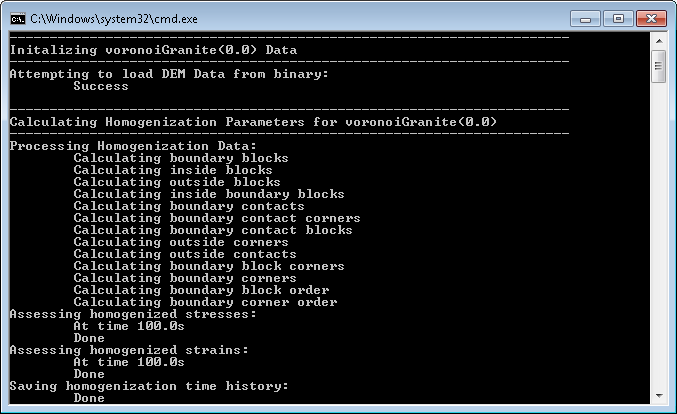
\includegraphics[width=\textwidth]{figures/Chapter4/HODSOutput}
\caption{{\label{fig:homCMD} MOUSE Outputs from HODS Module.%
}}
\end{center}
\end{figure}

